\begin{center}{ \bf  МНОГОУРОВНЕВОЕ МАТЕМАТИЧЕСКОЕ МОДЕЛИРОВАНИЕ ТЕПЛООБМЕНА В ЖИДКОСТНЫХ КАНАЛАХ ТЕРМОЭЛЕКТРИЧЕСКОГО БЛОКА ОХЛАЖДЕНИЯ\footnote{Работа выполнена при финансовой поддержке Министерства образования и науки Российской Федерации в рамках Федеральной целевой программы (Соглашение №14.577.21.0202, уникальный идентификатор RFMEFI57715X0202).}}\\
{\it Д.Н. Галдин, А.В. Кретинин, Е.Е. Спицына, И.В. Рощупкина} \\
\end{center}
\addcontentsline{toc}{section}{Галдин Д.Н., Кретинин А.В., Спицына Е.Е., Рощупкина И.В.\dotfill}

Моделирование компонента термоэлектрического блока охлаждения, по которому циркулирует жидкость, проводилось с использованием модуля вычислительной гидродинамики Ansys CFX.
В расчёте были использованы следующие модули Ansys Workbench:
\begin{itemize}
	\item
		ANSYS Design Modeler~--- для работы с трёхмерной геометрической моделью каналов блока охлаждения.
		Данный модуль является универсальным CAD-ре\-да\-к\-то\-ром с широким набором инструментов для создания новой геометрии, а также для разбиения и упрощения импортированной геометрии. Данный модуль в своей основе имеет ядро Parasolid, обладает надежным, отказоустойчивым генератором геометрии и соответствует производственным стандартам.
	\item
		ANSYS Meshing – для генерации сеточной модели по исходной модели проточной части. Модуль содержит широкий набор методов, удовлетворяющих специфическим требованиям той или иной области физики, а также мощный функционал управления глобальными параметрами и локальными сгущениями расчетной сетки (функции автоматического изменения размеров; локальные измельчения сетки по ребру, поверхности, в объеме; переменная плотность сетки).
	\item
		Ansys CFX - для расчётов гидрогазодинамики.
	\item
		Parameter Set – для задание входных параметров и сбора результатов расчётов.
\end{itemize}
Исходная модель моделируемого блока охлаждения представлена на рисунке 1. Для отображения внутренних компонентов из модели исключён внешний корпус. Блок охлаждения состоит из элементов Пельтье, жидкостного теплообменника и воздушного теплообменника.

\begin{figure}[h!]
	\centering
	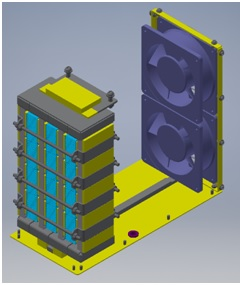
\includegraphics[width=0.9\textwidth]{gla1.jpg}
	\caption{Модель блока охлаждения}
\end{figure}

Далее приведен пример моделирования жидкостного те\-плообменника с граничными условиями
для одной точки из плана вычислительного эксперимента.
Моделирование проводилось в стационарной постановке.
В качестве граничных и начальных условий в моделируемом варианте постановки задачи использованы следующие значения:

- на входе в проточную часть (Рисунок 2) задавался массовый расход жидкости 0,01861 кг/с;
температура жидкости задавалась равной 46,7~$^\circ$С;

- на выходе из проточной части – среднее статическое давление 2 атм;

- температура на поверхностях теплообмена задавалась равной 30~$^\circ$С.

Суммарная площадь поверхности теплообмена 0,184433 м$^2$.

\begin{figure}[h!]
	\centering
	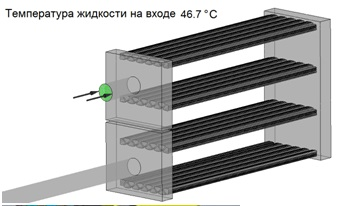
\includegraphics[width=0.9\textwidth]{gla2.jpg}
	\caption{Граничные условия на входе в проточную часть}
\end{figure}

В результате моделирования полученное среднее значение коэффициента теплоотдачи 369,082 [Вт/(м2•К)]. Распределение значения коэффициента теплоотдачи по поверхности теплообмена представлено на рисунке 3.

\begin{figure}[h!]
	\centering
	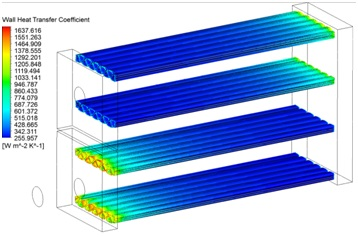
\includegraphics[width=0.9\textwidth]{gla3.jpg}
	\caption{Распределение значения коэффициента теплоотдачи по поверхности теплообмена}
\end{figure}


На основе обработки экспериментальных данных получены значения коэффициента теплоотдачи во всех точках плана эксперимента,
которые обеспечивают приемлемую то\-ч\-ность определения основных параметров функционирования ТЭМО.
На основе технологии Response Surface модуля ANSYS DesignXplore установлено,
что коэффициент теплоотдачи от жидкости в стенку зависит от 4 параметров:
\textit{I} - силы тока установку, $T_{f} \cdot T_{x} \cdot T_{g} $ - средних температур жидкости, холодной и горячей сторон ТЭМО на данном режиме.

Получена зависимость $\alpha _{6} (I,T_{f} ,T_{x} ,T_{g} )$, которая обеспечивает точность не менее 1.5 \% по определению коэффициента теплоотдачи от жидкости на холодной стороне ТЭМО.

\[
	\begin{array}{l}
		\alpha _{6} =-25.981755+73.2158396\cdot T_{x} -22.644839\cdot T_{f}+
		\\+
		2.61022986\cdot T_{x}^{2} + 1.28292285\cdot T_{f}^{2} -4.1723389\cdot T_{x} \cdot T_{f} +
		\\+
		74.2391083\cdot I-25.621\cdot T_{g} -0.14647315\cdot I^{2} +
		\\+
		0.104869597\cdot T_{g}^{2} -2.34\cdot I\cdot T_{f} +
		1.76037\cdot I\cdot T_{x} -
		\\-
		0.49132\cdot I\cdot T_{g} +
		0.56715222\cdot T_{f} \cdot T_{g} -
		\\-
		0.96986872\cdot T_{x} \cdot T_{g} +
		0.015616455\cdot I\cdot T_{f} \cdot T_{x} +
		\\+
		0.017657\cdot I\cdot T_{f} \cdot T_{g} -
		0.00252416\cdot I\cdot T_{x} \cdot T_{g} +
		\\+
		0.005895081\cdot T_{x} \cdot T_{f} \cdot T_{g} -
		\\-
		0.000297\cdot I\cdot T_{f} \cdot T_{x} \cdot T_{g}
	\end{array}
\]

Здесь \textit{I} - сила тока на всю установку, а $T_{f} \cdot T_{x} \cdot T_{g} $ - средние температуры жидкости, холодной и горячей сторон ТЭМО на данном режиме.

Данная зависимость может быть использована в расчетных моделях теплообмена,
полученных в виде критериальных соотношений Nu=\textit{f}(Re,Pr),
что в дальнейшем позволяет проводить расчеты без привлечения инструментария ANSYS.

При процедуре моделирования большое значение имеет выбор уровня «точности». Быстрый расчет, основанный на одномерных методах и эмпирических данных, позволяет оперативно реагировать на изменения на системном уровне, однако имеет невысокую точность. С другой стороны, полноценные 3D-методы обеспечивают более высокий уровень точности и снижение уровня эпистемических неопределенностей, связанных с инструментами моделирования. Ключевым моментом, определяющим эффективность процесса управления неопределенностями, является применение высокоточных методов моделирования, основанных на совокупности применяемых физических законов с последующим их использованием при выполнении оптимизации в рамках робастного проектирования. В связи с этим все рабочие процессы в ТЭБО моделировались с использованием математических моделей самого высокого иерархического уровня на основе инструментария платформы ANSYS Workbench, а затем результаты моделирования обобщались с использованием технологии Response Surface до вида аппроксимационных полиномиальных зависимостей.

\smallskip \centerline{\bf Литература}\nopagebreak

1. {\it Kamil Lubikowski, Stanislaw Radkowskia, Krzysztof
\linebreak
Szczurowskia, Michal Wikarya}
\foreignlanguage{english}{
	Seebeck phenomenon, calculation method comparison. Journal of Power Technologies 95 (Polish Energy Mix), 2015. - 63–67.
}

2. \foreignlanguage{english}{
	{\it D. Enescu, E.O. Virjoghe, M. Ionel, M.F. Stan} Electro-thermal analysis of peltier cooling using FEM.Scientific Bulletin of the Electrical Engineering Faculty – Year 10 No. 1 (12)
}

3. \foreignlanguage{english}{
	Development of an experimental and analytical model of an active cooling method for high-power three-dimensional integrated circuit (3d-ic) utilizing multidimensional configured thermoelectric modules, HUY NGOC PHAN, PhD Thesis, the university of Texas at Arlington, 2011.
}
